\chapter{Rigidity: An Introduction} % previously Definitions \& Preliminaries

\begin{flushleft}
Rigidity can be easily understood as observing a structure and questioning how 'stiff' it is. If some force is applied to it, does it bend or buckle? When we pull the structure across (Euclidean) space, do we move it entirely, or does a part of it bend and move in the direction of the pull? As stiffness can be interpreted in a multitude of ways, this section will be dedicated to formalizing the definition of rigidity that we will use for the remainder of this project. 
\end{flushleft}

\begin{flushleft}
To start, we must first understand what \textit{graphs} are.
\end{flushleft}

\section{Graph Theory}

\begin{flushleft}
Here, we delve into a small portion of a very large field of mathematics. The definitions presented here will be fundamental for what's to come.
\end{flushleft}

\begin{definition}
    A \textit{graph} $G = (V,E)$ consists of a set V and a set E of two-element subsets of V. The elements of V are called \textit{vertices} and the elements of E are called \textit{edges}.
\end{definition}

\begin{example}
The graph $G = (V,E)$ below
\label{eg: cycle}
\begin{figure}[ht]
    \centering
    \documentclass{standalone}
\usepackage{tikz}
\usetikzlibrary{arrows,backgrounds,positioning,petri, calc}


\begin{document}
% Set the style for the vertices
\tikzstyle{vertex} = [circle, draw=black, fill = black, thin, inner sep=0pt,minimum size=2mm]

\begin{tikzpicture}
    
    % Define nodes
    \node (1) at (0,0) [vertex, label=left:$1$] {};
    \node (2) at (1,1) [vertex, label=above:$2$] {};
    \node (3) at (2.5,1) [vertex, label=above:$3$] {};
    \node (4) at (2.5,-1) [vertex, label=below:$4$] {};
    \node (5) at (1,-1) [vertex, label=below:$5$] {};

    % add edges
    \path[] (1) edge (2)
                edge (5)
            (3) edge (2)
                edge (4)
            (4) edge (5);
    
\end{tikzpicture}
\end{document}

% when entering figures, use the following format

%\begin{figure}[htbp]
%    \centering
%    \input{Chapter 1/framework}
%    \caption{Caption}
%    \label{fig:enter-label}
%\end{figure}
    \label{simple graph}
\end{figure}
\noindent
has $|V| = 5$, and $|E| = 5$.
\end{example}

\begin{definition}
A graph $G$ is \textit{connected} if for any two vertices $u,v$, there exists a sequence of distinct vertices (called a \textit{path}) $u_1, \hdots, u_k$, such that $u_iu_{i+1}$ is an edge of $G$ for $0 \leq i \leq k-1$ that connect $u$ and $v$. The path can be seen as 

\[
u = u_0, u_1, \hdots, u_{k-1}, u_k = v
\]
\end{definition}

\begin{definition}
A \textit{cycle} is a graph $G = (V,E)$  where $G$ has $n$ vertices, and the edges are 

\[
E(G) = \{12, 23, \hdots, (n-1)n \}
\]

\noindent
It can be thought of as a closed path. 
\end{definition}

\begin{example}
The graph in Example \ref{eg: cycle} is a cycle of length 5.
\end{example}

\begin{definition}
The \textit{degree} of a vertex is the number of edges incident to the vertex.
\end{definition}

\begin{flushleft}
There are several ways of drawing the 'same' graph on the plane. This includes labelling them in a variety of ways as well. Therefore, it is vital that we class these drawings as the same graph.
\end{flushleft}

\begin{definition}
\label{def: isomorphism}
Two graphs $G_1$ and $G_2$ are said to be \textit{isomorphic} if there is a bijection $\phi$ : $V(G_1) \rightarrow V(G_2)$ such that $xy \in E(G_1)$ if and only if $\phi(x)\phi(y) \in E(G_2)$. The function $\phi$ is known as an \textit{isomorphism}.
\end{definition}

\begin{example}
\label{eg: isomorphic graphs}
Consider the two graphs below.

\begin{figure}[ht]
    \centering
    \documentclass{standalone}
\usepackage{tikz}
\usetikzlibrary{arrows,backgrounds,positioning,petri, calc}


\begin{document}
% Set the style for the vertices
\tikzstyle{vertex} = [circle, draw=black, fill = black, thin, inner sep=0pt,minimum size=2mm]

\begin{tikzpicture}
    
    % Define nodes for the first K4
    \node (11) at (0,0) [vertex, label=below:$1$] {};
    \node (12) at (0,2) [vertex, label=above:$2$] {};
    \node (13) at (2,2) [vertex, label=above:$3$] {};
    \node (14) at (2,0) [vertex, label=below:$4$] {};
    \node[draw = none] (G1) at (1,-1) [label=above:$G_1$] {};

    % define nodes for the second K4
    \node (21) at (4,0) [vertex, label=below:$a$] {};
    \node (22) at (4,2) [vertex, label=above:$b$] {};
    \node (23) at (6,2) [vertex, label=above:$c$] {};
    \node (24) at (6,0) [vertex, label=below:$d$] {};
    \node[draw = none] (G1) at (5,-1) [label=above:$G_2$] {};

    % add the edges
    \path[] (11) edge (12)
                edge (14)
            (12) edge (13)
            (13) edge (11); 

    \path[] (21) edge (23)
            (22) edge (23)
                edge (24)
            (23) edge (24);
\end{tikzpicture}
\end{document}
    %\caption{Caption}
    \label{fig:isomoprhic graphs}
\end{figure}
\vspace{-5 mm}
\begin{flushleft}
The bijection $\phi : G_1 \rightarrow G_2$ is given by $\phi(1) = c$, $\phi(2) = b$, $\phi(3) = c$, and $\phi(4) = a$.    
\end{flushleft}
\end{example}

\begin{flushleft}
Given a graph $G$, we may be interested in a certain subset of vertices and edges that are included in $G$. This involves studying a \textit{subgraph} of $G$.
\end{flushleft}

\begin{definition}
A graph $H$ is a \textit{subgraph} of $G$ if there is a graph $H'$ isomorphic to $H$ such that $V(H') \subseteq V(G)$ and $E(H') \subseteq E(G)$.
\end{definition}

\begin{example}
Consider the graphs below.

\begin{figure}[ht]
    \centering
    \documentclass{standalone}
\usepackage{tikz}
\usetikzlibrary{arrows,backgrounds,positioning,petri, calc}


\begin{document}
% Set the style for the vertices
\tikzstyle{vertex} = [circle, draw=black, fill = black, thin, inner sep=0pt,minimum size=2mm]

\begin{tikzpicture}
    
    % Define nodes
    \node (1) at (0,0) [vertex, label=left:$1$] {};
    \node (2) at (1,1) [vertex, label=above:$2$] {};
    \node (3) at (3,1) [vertex, label=above:$3$] {};
    \node (4) at (3,-1) [vertex, label=below:$4$] {};
    \node (5) at (1,-1) [vertex, label=below:$5$] {};
    \node[draw = none] (G1) at (2,-2.25) [label=above:$G$] {};

    \node (21) at (6,0) [vertex, label=left:$1$] {};
    \node (22) at (7,1) [vertex, label=above:$2$] {};
    \node (25) at (7,-1) [vertex, label=below:$5$] {};
    \node[draw = none] (H) at (7,-2.25) [label=above:$H$] {};
    

    % add edges
    \path[] (1) edge (2)
                edge (5)
            (3) edge (2)
                edge (4)
            (4) edge (5)
            (2) edge (5)
            (21) edge (22)
                edge (25)
            (22) edge (25);
    
\end{tikzpicture}
\end{document}

    %\caption{Caption}
    %\label{fig:enter-label}
\end{figure}
\noindent
Here, as $V(H) \subseteq V(G)$ and $E(H) \subseteq E(G)$, it follows that $H$ is a subgraph of $G$.
\end{example}

\begin{flushleft}
The last idea we need from graph theory is the notion of \textit{planarity}. The graphs we are interested in for this project are those such that the edges do not cross over each other.
\end{flushleft}

\begin{definition}
    \label{def: planar graphs}
    A graph $G$ is \textit{planar} if it has a drawing in the plane such that none of edges cross over each other.
\end{definition}

\begin{example}
    Consider \hyperref[eg: isomorphic graphs]{Example \ref*{eg: isomorphic graphs}}. The graph $G_1$ is a planar drawing of the graph $G_2$.
\end{example}

\section{Frameworks}

\begin{flushleft}
    Now that we have a good idea of what graphs are, we can start working on setting up frameworks. The definitions in this section will be defined in the space $\mathbb{R}^d$, where $d \in \mathbb{N}$. Later, we will find ourselves working exclusively in $\mathbb{R}^2$. For the remainder of this chapter, we shall adhere closely to the contents in chapter 2 from the book ``Frameworks, Tensegrities, and Symmetry'' by Robert Connelly and Simon D. Guest \cite{textbook}.
    % better way of wriitng this para?
    
    The first definition we need is that of a \textit{configuration}.
\end{flushleft}

\begin{definition}
    Suppose we have a collection of $n$ labelled points in $\mathbb{R}^d$, where $d \in \mathbb{N}$. Let $\mathbf{p}_i = (p_{i1}, \hdots, p_{id})$ be the position vector of point $i$. Then a \textit{configuration} is

\[
\mathbf{p} = (\mathbf{p}_1, \hdots, \mathbf{p}_n),
\]

\begin{flushleft}
where $\mathbf{p}$ is a vector of vectors in $\mathbb{R}^d$.     
\end{flushleft}
\end{definition}

\begin{flushleft}
Therefore, a configuration can be thought of as a set of points in the space $\mathbb{R}^d$, each point equipped with its own position vector. Henceforth, we will refer the the points in a configuration as \textit{nodes}. 
\end{flushleft}

\begin{flushleft}
Given a configuration, we can now decide which pairs of nodes to connect with a graph $G$. The nodes in $\mathbf{p}$ correspond to the vertices in $G$, and $G$ is not allowed to have multiple edges between vertices, or loops between the same vertex (such graphs are known to be \textit{simple}).
\end{flushleft}

\begin{definition}
    A \textit{framework} is a configuration $\mathbf{p} = (\mathbf{p}_1, \hdots, \mathbf{p}_n)$ together with its corresponding graph $G = (V,E)$. We denote it as $(G,\mathbf{p})$.
\end{definition}

%** IS THIS NEEDED?
\begin{flushleft}
Note that as we are working in $\mathbb{R}^d$, the \textit{length} of each edge with endpoints $\mathbf{p}_i$ and $\mathbf{p}_j$ in a framework $(G,\mathbf{p})$ is the \textit{Euclidean distance} between the points $\mathbf{p}_i$ and $\mathbf{p}_j$. This is denoted $|\mathbf{p}_i - \mathbf{p}_j|$.

In this project, graphs will be drawn with vertices that are filled in, whereas frameworks will have hollow nodes. 
\end{flushleft}

%\clearpage

\begin{example}
\label{g vs f}
In the two diagrams below, the one on the left is a graph, whereas the one on the right is a framework.
    \begin{figure}[h]
        \centering
        \documentclass{standalone}
\usepackage{tikz}
\usetikzlibrary{arrows,backgrounds,positioning,petri, calc}


\begin{document}
% Set the style for the vertices
\tikzstyle{vertex} = [circle, draw=black, thin, inner sep=0pt,minimum size=2mm]

\begin{tikzpicture}
    
    % Define nodes for the first K4
    \node (11) at (0,0) [vertex, fill = black] {};
    \node (12) at (0,2) [vertex, fill = black] {};
    \node (13) at (2,2) [vertex, fill = black] {};
    \node (14) at (2,0) [vertex, fill = black] {};

    % add invisible node at (1,-1)
    \node[draw = none] (graph) at (1, -.5) {Graph};

    % define nodes for the second K4
    \node (21) at (4,0) [vertex] {};
    \node (22) at (4,2) [vertex] {};
    \node (23) at (6,2) [vertex] {};
    \node (24) at (6,0) [vertex] {};

    \node[draw = none] (graph) at (5, -.5) {Framework};

    % add the edges
    \path[] (11) edge (12)
                edge (14)
            (12) edge (13)
            (13) edge (11)
                edge (14); 

    \path[] (21) edge (22)
                edge (24)
            (22) edge (23)
            (23) edge (21)
                edge (24); 
\end{tikzpicture}
\end{document}
    \end{figure}
\end{example}
\vspace{-8 mm}
\begin{flushleft}
At this stage, you may be wondering what exactly the difference between a graph and a framework is. Put simply,
\begin{itemize}
    \item A graph is an abstract mathematical object that can be visualised in a multitude of ways, as seen in \hyperref[eg: isomorphic graphs]{Example \ref*{eg: isomorphic graphs}}. Varying the edge lengths does not produce a new graph as by \hyperref[def: isomorphism]{Definition \ref*{def: isomorphism}}, they are isomorphic, and considered the `same'.
    \vspace{-3mm}
    \item In a framework however, we are fixing points in space. If we consider a framework in $\mathbb{R}^2$ such as the one in \hyperref[g vs f]{Example \ref*{g vs f}}, each node is at a determined distance from each other. Slightly changing the position of a node results in a different framework.

\end{itemize}
\end{flushleft}

\begin{flushleft}
Frameworks are essential when it comes to studying the rigidity of structures. Considering real-world applications, a simple model of a building can be designed by considering what its framework would look like in $\mathbb{R}^3$. Investigating this framework allows for insight into how the building in question should be built.
\end{flushleft}

\noindent
Armed with the notion of a framework, we can begin thinking about how we might be able to change the shape of a framework. 

\section{Motions}

\begin{flushleft}
When it comes to studying the rigidity of frameworks, we begin by understanding what it means for a framework to experience a \textit{motion} (also known as a \textit{flex}). 
\end{flushleft}

\begin{definition}
Suppose the configuration $\mathbf{p} \in \mathbb{R}^d$ is on a differentiable smooth path parameterized by time $t$, denoted $\mathbf{p}(t)$. Then 

    \begin{itemize}
        \item The position of node $\mathbf{p}_i \in \mathbf{p}$ at any time $t$ is given by $\mathbf{p}_i(t) \in \mathbb{R}^d$.
        \vspace{-3mm}
        \item The \textit{initial position} of a node $\mathbf{p}_i$ is $\mathbf{p}_i(0) \in \mathbb{R}^d$
        \vspace{-3mm}
        \item The \textit{initial configuration} of $\mathbf{p}$ is 
        \[
        \mathbf{p}(0) = (\mathbf{p}_1(0), \hdots, \mathbf{p}_n(0) \in \mathbb{R}^{nd}
        \]
    \end{itemize}
\end{definition}

\begin{definition}
A \textit{motion} of the framework $(G,\mathbf{p})$ is a path $\mathbf{p}(t)$ such that 

\[
|\mathbf{p}_i(t) - \mathbf{p}_j(t)| = |\mathbf{p}_i(0) - \mathbf{p}_j(0)|,
\]

\noindent
for all $t$, and for all $ij \in E(G)$.
\end{definition}

\begin{flushleft}
In other words, a motion preserves the length of every edge in the framework at any point in time. A motion $\mathbf{p}(t) = (\mathbf{p}_1(t), \hdots, \mathbf{p}_n(t))$ is a \textit{continuous motion} if each of the $d$ coordinates of $\mathbf{p}_i(t)$ is continuous in $t$. This simply means that the nodes of the configuration should follow an uninterrupted path in $\mathbb{R}^d$ with respect to time. 
\end{flushleft}

\begin{flushleft}
There are certain motions that we can apply to a framework such that the distances between all the nodes are preserved as well. Such motions are known as \textit{rigid motions}.
\end{flushleft}

\begin{definition}
A \textit{rigid motion} of the framework $(G,\mathbf{p})$ is a path $\mathbf{p}(t)$ such that 

\[
|\mathbf{p}_i(t) - \mathbf{p}_j(t)| = |\mathbf{p}_i(0) - \mathbf{p}_j(0)|,
\]

\noindent
for all $t$, and for all $i, j \in V(G)$
\end{definition}

\begin{flushleft}
From this definition, we can see that there are only two ways in which a motion can be classed as a rigid motion.     
\end{flushleft}

\begin{itemize}
    \item \textit{Translating} the entire framework across $\mathbb{R}^d$ preserves the distances between each node, and so it is a rigid motion.
    \vspace{-3mm}
    \item \textit{Rotating} the entire framework about a point also preserves the distances between each node. Thus, it is a rigid motion as well.
    \vspace{-3mm}
\end{itemize}

\begin{flushleft}
In order to formalize this, we let the matrix $\mathbf{Q}(t)$ describe a rotation of a node in $\mathbb{R}^d$, where $\mathbf{Q}(0)$ is the identity matrix, and we let $\mathbf{w}(t)$ be a translation of a node in $\mathbb{R}^d$, where $\mathbf{w}(0)$ is the zero vector. Then we can classify all rigid motions as paths of each node $\mathbf{p}_i(t)$ that have the form 

\[
\mathbf{p}_i(t) = \mathbf{Q}(t)\mathbf{p}_i + \mathbf{w}(t)
\]

Thus, rotating and translating a framework in any order is always a rigid motion.
\end{flushleft}

\begin{example}
\label{eg: simple motion}
Consider the framework with 3 nodes, labelled $1,2,3$, and two edges, $12$, and $23$. Apply the motion 

\[ p_i(t) = 
\begin{cases}
    \cos(t) - \sin(t), & \text{if } i = 3 \\
    p_i(0), & \text{if } i = 1,2
\end{cases}
\]

\vspace{3 mm}
\noindent
to this framework. A diagram of what happens for times $t=0$, and $t=1$ is shown below
%\clearpage

    \begin{figure}[htbp]
        \centering
        \documentclass{standalone}
\usepackage{tikz}
\usetikzlibrary{arrows,backgrounds,positioning,petri, calc}

\begin{document}
% Set the style for the vertices
\tikzstyle{vertex} = [circle, draw=black, thin, inner sep=0pt,minimum size=2mm]

\begin{tikzpicture}

    % before the motion
    \node (11) at (0,0) [vertex, label=above:$\textbf{p}_1$] {};
    \node (12) at (2,0) [vertex, label=above:$\textbf{p}_2$] {};
    \node (13) at (2,-2) [vertex, label=below:$\textbf{p}_3$] {};

    \node[draw = none] (t1) at (-0.2, -1.5) {$t = 0$};
    %\draw[->] (2.5,-1) -- (4.5,-1);
    % after the motion
    \node (21) at (5,0) [vertex, label=above:$\textbf{p}_1$] {};
    \node (22) at (7,0) [vertex, label=above:$\textbf{p}_2$] {};
    \node (23) at (5.6, -1.4) [vertex, label = below: $\textbf{p}_3$] {};

    \node[draw = none] (t2) at (4.5, -1) {$t = 1$};

    % add the edges before the motion
    \path[] (11) edge (12);
    \path[] (12) edge (13); % Make this edge red
    
    % Swing node (13) along an arc towards node (11)
    \path[draw, ->, dashed] (13) edge [bend left = 40] (11); 

    % add the edges before the motion
    \path[] (21) edge (22);
    \path[] (22) edge (23); % Make this edge red
    
    % Swing node (13) along an arc towards node (11)
    \path[draw, ->, dashed] (23) edge [bend left = 20] (21); 

\end{tikzpicture}
\end{document}

        \caption{A framework where the edge $23$ can swing about $2$.}
        \label{fig: simple motion}
    \end{figure}
\vspace{-5 mm}
\begin{flushleft}
As all the edge lengths are preserved, this is a motion. However, the distance between nodes $1$ and $3$ changes as $t$ changes. Therefore, this is not a rigid motion.    
\end{flushleft}
\end{example}

\begin{example}
Consider the matrix 

\[ \mathbf{Q} = 
\begin{pmatrix}
-1 & 0\\
0 & -1\\
\end{pmatrix}
\]

\begin{flushleft}
This results in a rotation of each node by 180$\degree$ about the origin $O$ in $\mathbb{R}^2$. Applying this to a framework at $t = 0$ in \hyperref[eg: simple motion]{Example \ref*{eg: simple motion}}, we obtain

\begin{figure}[htbp]
    \centering
    \documentclass{standalone}
\usepackage{tikz}
\usepackage{gensymb}
\usetikzlibrary{arrows,backgrounds,positioning,petri, calc}

\begin{document}
% Set the style for the vertices
\tikzstyle{vertex} = [circle, draw=black, thin, inner sep=0pt,minimum size=2mm]

\begin{tikzpicture}[node distance = 2cm, auto, scale = 1]

    %\tikzstyle{every node}=[font=\small]

    % before the motion
    \node (11) at (-1,0) [vertex, label=above:$\textbf{p}_1$] {};
    \node (12) at (1,0) [vertex, label=above:$\textbf{p}_2$] {};
    \node (13) at (1,-2) [vertex, label=below:$\textbf{p}_3$] {};

    % add node for the origin
    \node (origin) at (0,-1) [vertex, fill = black, label=below:$O$] {};

    % add an invisble node
    \node[draw = none] (start) at (1.2, -1) {};

    % add an invisible node for the label
    \node[draw = none] (label) at (3.5, -1)[label=above:Multiply by $\mathbf{Q}$]{};

    % after the motion
    \node (21) at (8,-2) [vertex, label=below:$\textbf{p}_1$] {};
    \node (22) at (6,-2) [vertex, label=below:$\textbf{p}_2$] {};
    \node (23) at (6, 0) [vertex, label = above: $\textbf{p}_3$] {};

    % add node for the origin
    \node (origin2) at (7, -1) [vertex, label = above: $O$, fill = black] {};

    % add an invisble node
    \node[draw = none] (end) at (5.8, -1) {};

    % add the edges before the motion
    \path[] (11) edge (12);
    \path[] (12) edge (13); % Make this edge red
    
    % add the edges before the motion
    \path[] (21) edge (22);
    \path[] (22) edge (23);  

    % plot the line between the diagrams
    \draw[->] (start) -- (end);
    

\end{tikzpicture}
\end{document}

\end{figure}

As all the edge lengths, as well as the distances between each node are preserved, this is a rigid motion.    
\end{flushleft}
\end{example}

\section{Rigidity}
\begin{flushleft}
As we have seen, rigid motions maintain not only the lengths of every edge in a framework, but they also fix the distance between each node as well. At this stage, we can question what frameworks can only be subject to rigid motions. Is there a framework such that the only way to move it is if we move \textit{all} of it?

The answer is yes, and such frameworks are said to be \textit{rigid}.
\end{flushleft}

\begin{definition}
\label{def: rigid}
A framework $(G,\mathbf{p})$ is rigid if every continuous motion $\mathbf{p}(t) = (\mathbf{p}_1(t), \hdots, \mathbf{p}_n(t))$ is a rigid motion. 
If a framework is not rigid, it is said to be \textit{flexible}.
\end{definition}

\begin{example}
\label{eg: rigid graphs}    
These two frameworks are rigid.
\begin{figure}[htbp]
    \centering
    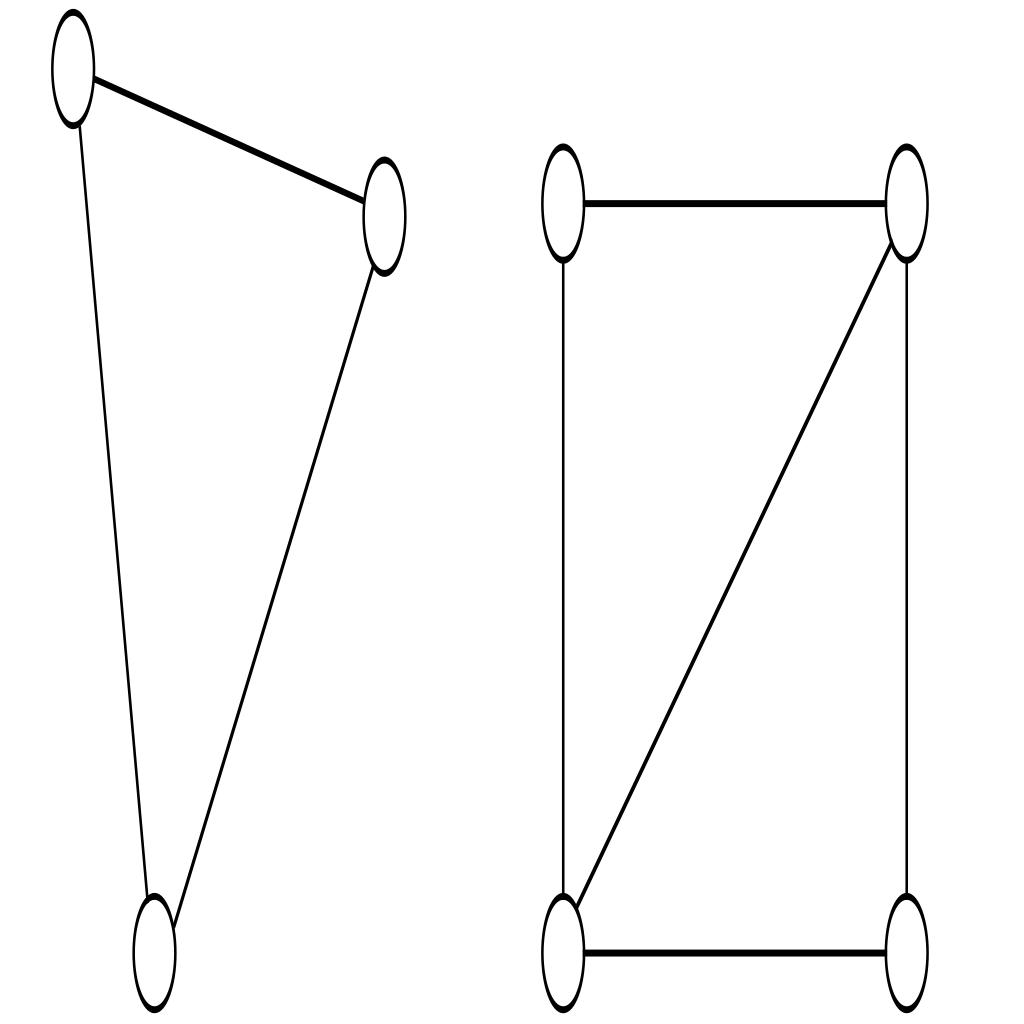
\includegraphics[width=0.57\textwidth]{Chapter 2/7. rigid_graphs.png} 
    \caption{Two rigid frameworks in $\mathbb{R}^2$}
    \label{fig: rigid_graphs}
\end{figure}
\begin{flushleft}
However, the following framework is not. We can apply a motion to the two nodes at the top such that the edge lengths are preserved, but the distance between the diagonal nodes change, violating the definition of rigidity.    
\end{flushleft}

\begin{figure}[htbp]
    \centering
    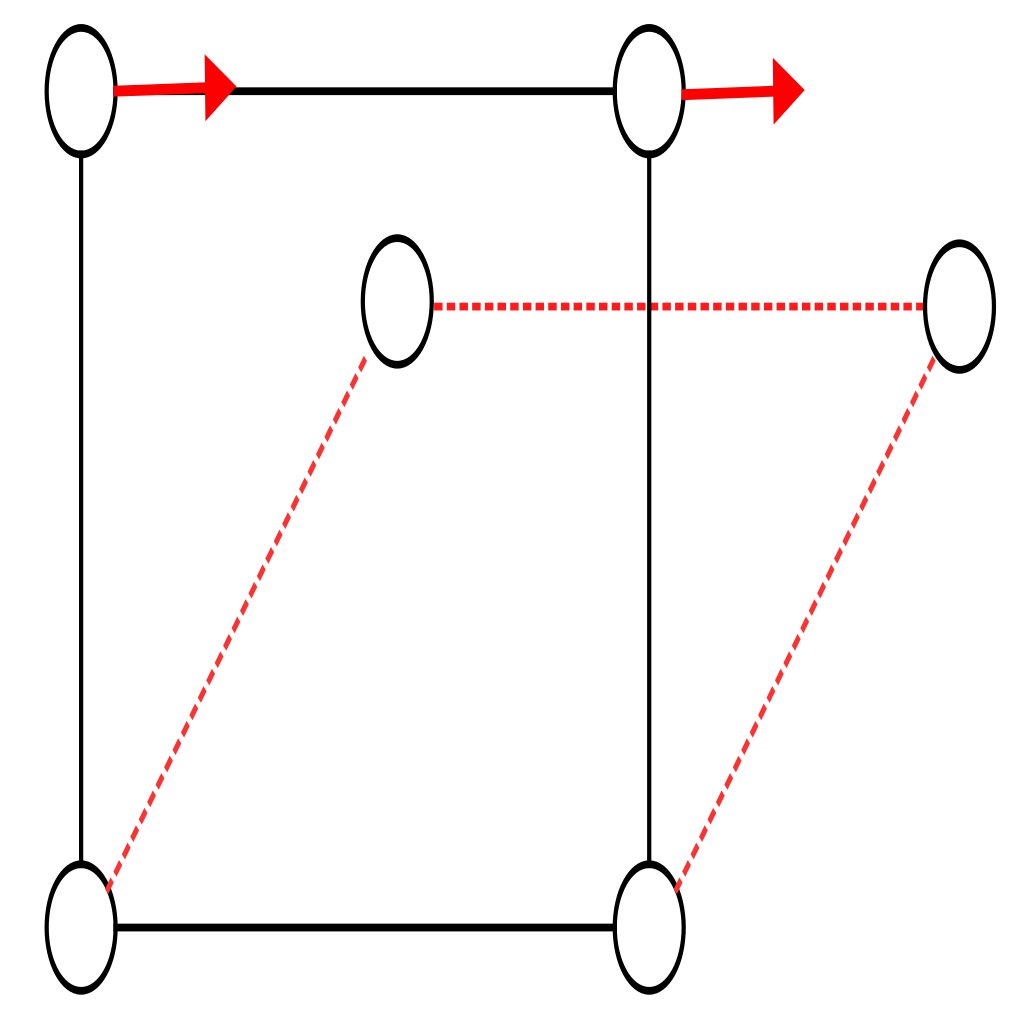
\includegraphics[width = 0.4\textwidth]{Chapter 2/8. not_rigid.png}
    \caption{A framework that is not rigid in $\mathbb{R}^2$}
    \label{eg: not_rigid}
\end{figure}
\end{example}
\vspace{-5 mm}
\begin{flushleft}
Another equivalent definition that was proved by Asimow and Roth \cite{asimow} that uses ideas of the congruency of frameworks.
\end{flushleft}

\begin{definition}
Consider two frameworks $(G,\mathbf{p})$ and $(G,\mathbf{q})$ where $\mathbf{p} = (\mathbf{p}_1, \hdots, \mathbf{p}_n)$ and $\mathbf{q} = (\mathbf{q}_1, \hdots, \mathbf{q}_n)$.
\begin{itemize}
    \item $\mathbf{q}$ is \textit{equivalent} to $\mathbf{p}$ if $|\mathbf{p}_i - \mathbf{p}_j| = |\mathbf{q}_i - \mathbf{q}_j|$ for all $ij \in E(G)$.
    \vspace{-3mm}
    \item $\mathbf{q}$ is \textit{congruent} to $\mathbf{p}$ if $|\mathbf{p}_i - \mathbf{p}_j| = |\mathbf{q}_i - \mathbf{q}_j|$ for all $i, j \in V(G)$.
\end{itemize}
\end{definition}

\begin{flushleft}
To put it another way, two frameworks $(G,\mathbf{p})$ and $(G,\mathbf{q})$ are equivalent if the edge lengths are the same for every pair of labelled nodes in $(G,\mathbf{p})$.

They are congruent if $(G,\mathbf{p})$ can be obtained through a series of rotations and translations of $(G,\mathbf{q})$. 
\end{flushleft}

% come up with a good diagram for the following definition. I am thinking of a framework with an epsilon circle around it, similar to hakan phd, but an equivalent framework with nodes in different places in this epsilon circle. Ask Louis?
% https://www.youtube.com/watch?v=kQlrqrjBXtk, 3:03
\begin{definition}
A framework $(G,\mathbf{p})$ on $n$ nodes is \textit{rigid} if there exists an $\epsilon>0$ such that for every configuration $\mathbf{q}$, where $(G,\mathbf{q})$ is equivalent to $(G,\mathbf{p})$, satisfies 

\[
|\mathbf{p}_i - \mathbf{q}_i| < \epsilon
\]
\begin{flushleft}
for all $i \in V(G)$, and is congruent to $(G,\mathbf{p})$.  
\end{flushleft}
\end{definition}

\begin{figure}[htbp]
    \centering
    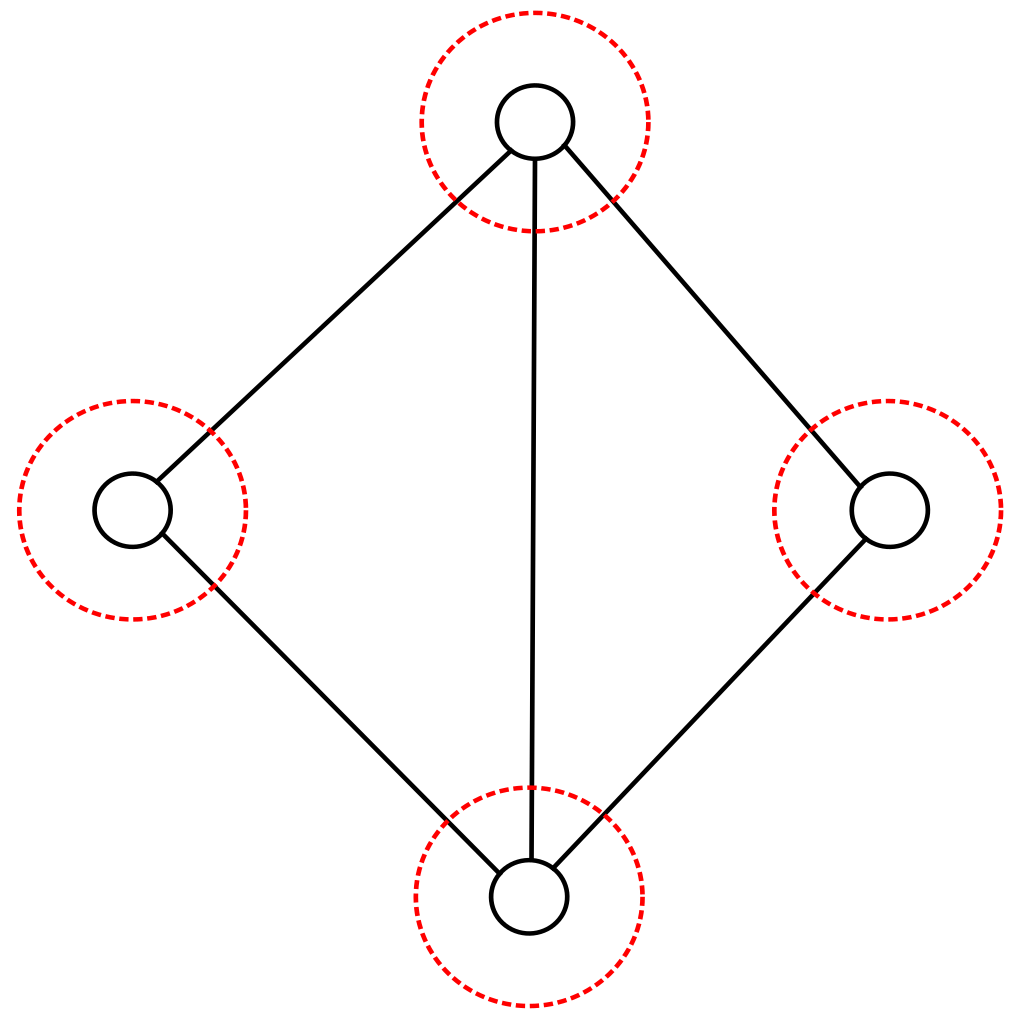
\includegraphics[width = 0.35\textwidth]{Chapter 2/14. epsilon.png}
    \caption{A framework $\mathbf{p}$ with an epsilon bound (red) for every node}
    \label{fig: epsilon}
\end{figure}
\vspace{-3mm}
\begin{flushleft}
In Figure \ref{fig: epsilon}, we visualise what an epsilon bound for every node looks like. If we create a configuration $\mathbf{q}$ such that it is equivalent to the framework $\mathbf{p}$ in the figure, and the nodes of $\mathbf{q}$ fall within the epsilon bounds of each node in $\mathbf{p}$, then we are able to conclude that with some rigid motion, we are able to achieve congruence between $\mathbf{p}$ and $\mathbf{q}$. 

In such scenarios, equivalence implies congruence.    
\end{flushleft}

% https://www.youtube.com/watch?v=kQlrqrjBXtk
% 8:30
\subsection{Infinitesimal Rigidity}

\begin{flushleft}
In some sense, the definition of rigidity seems quite loose. Depending on the material used to construct the edges of the framework, we may be able to deform the edges. 
\end{flushleft}

\begin{figure}[htbp]
    \centering
    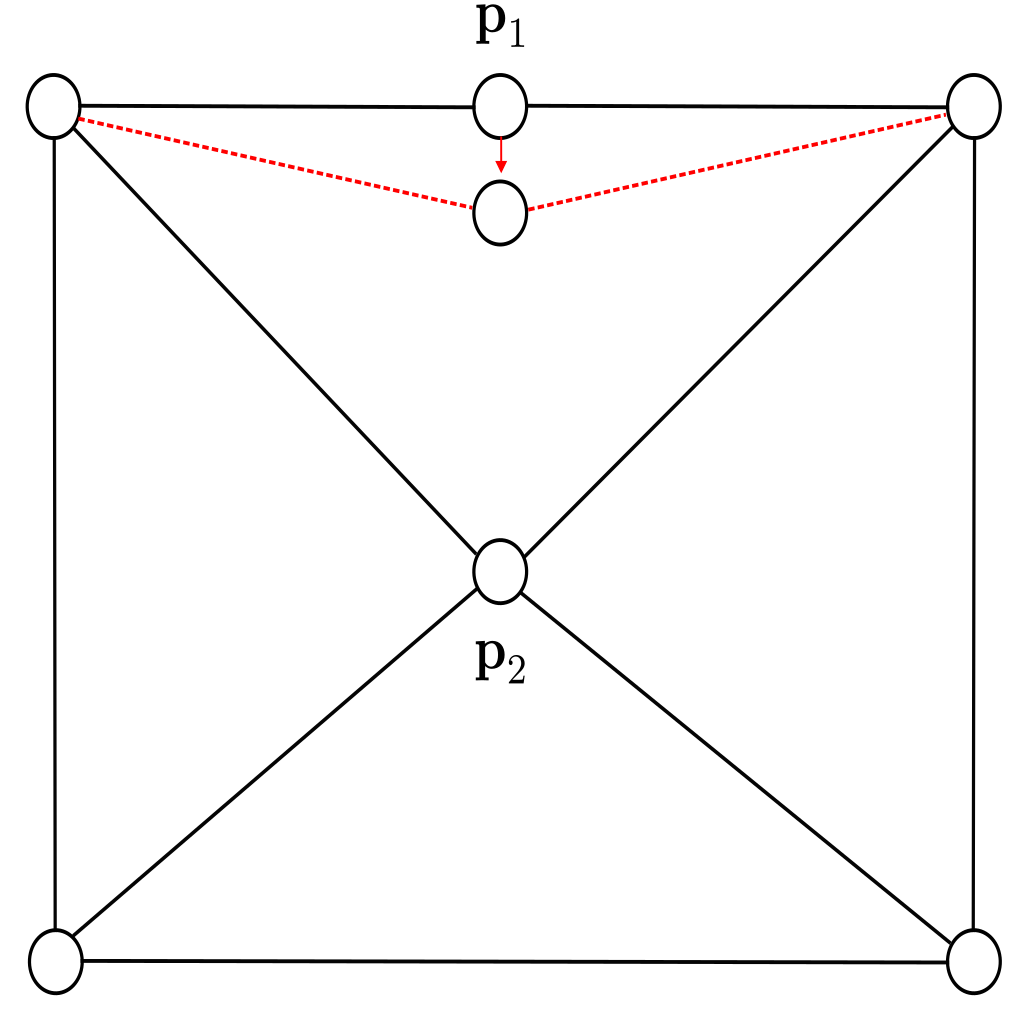
\includegraphics[width = 0.32\textwidth]{Chapter 2/9. not_inf_rigid.png}
    \caption{A framework with all nodes pinned, and an edge that can be displaced.}
    \label{fig: not_inf_rigid}
\end{figure}
\vspace{-2 mm}
\begin{flushleft}
Looking at Figure \ref{fig: not_inf_rigid}, if we consider the dotted edge to be a piece of string tied between two fixed nodes, then we can apply some force and deform the structure. Although the initial framework is rigid, it somehow doesn't `feel' rigid.
\end{flushleft}

\begin{flushleft}
In order to strengthen the definition of rigidity, let us first start with an observation described in greater detail by Graver in his book ``Counting on Frameworks'' \cite{counting_frameworks}. 
\end{flushleft}

\begin{flushleft}
Suppose that the configuration $\mathbf{p}$ is on a smooth differentiable path parameterized by time $t$. Consider a node of the configuration $\mathbf{p}_i$. Then its position is given by $\mathbf{p}_i(t)$ and as $\mathbf{p}_i$ is on a differentiable path, its derivative is well-defined.

\begin{figure}[htbp]
    \centering
    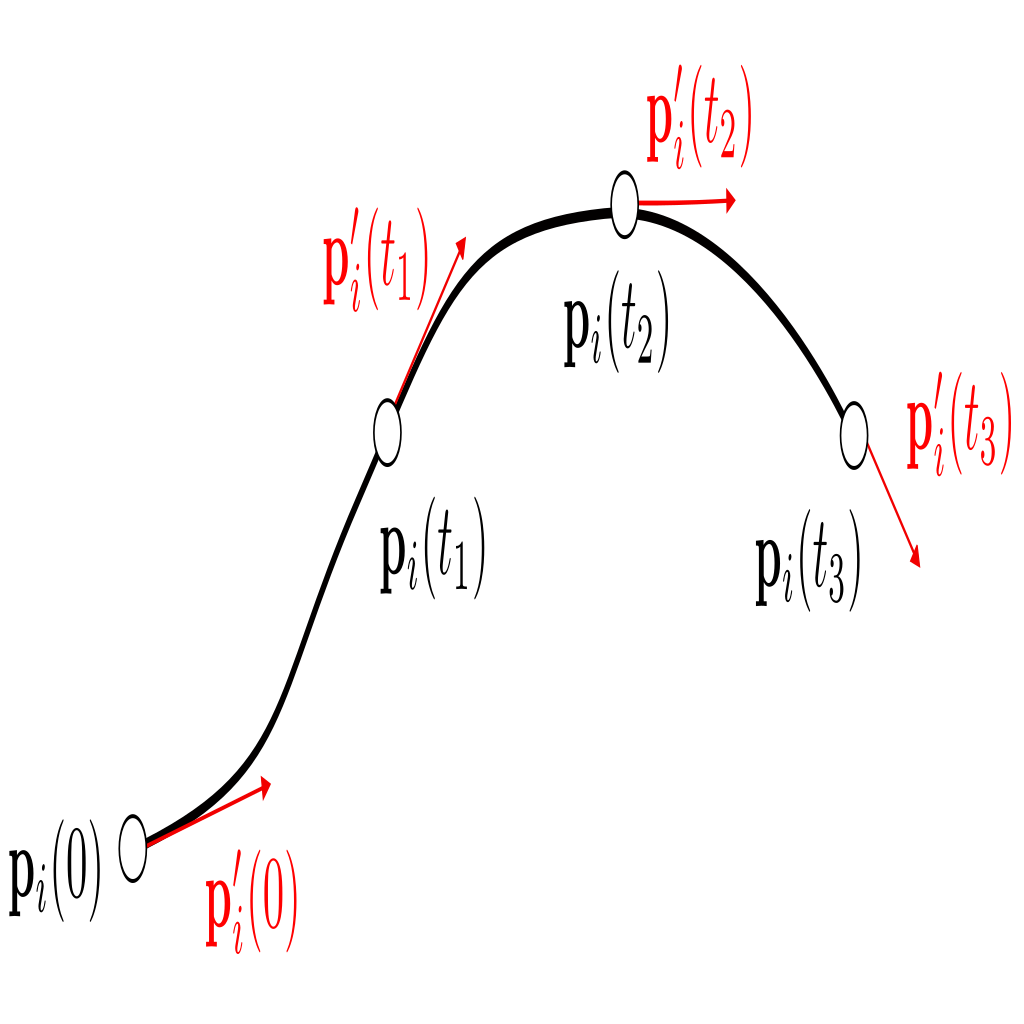
\includegraphics[width = 0.5\textwidth]{Chapter 2/12. path.png}
    \caption{Node $\mathbf{p}_i$ at various positions on path $\mathbf{p}_i(t)$ for various times $t$. The instantaneous velocities at each position $\mathbf{p}'_i(t)$ are marked in red}
    \label{fig: path}
\end{figure}
\end{flushleft}

\noindent
Taking the derivative of $\mathbf{p}_i(t)$ with respect to time gives us the instantaneous velocity $\mathbf{p}'_i(t)$ of the node $\mathbf{p}_i$ at time $t$.
%\vspace{-5.5 mm}

\begin{flushleft}
The velocities $\mathbf{p}'_i(t)$ become vital when studying infinitesimal rigidity. To motivate this, let us consider a framework in $\mathbb{R}^2$.

\begin{figure}[htbp]
    \centering
    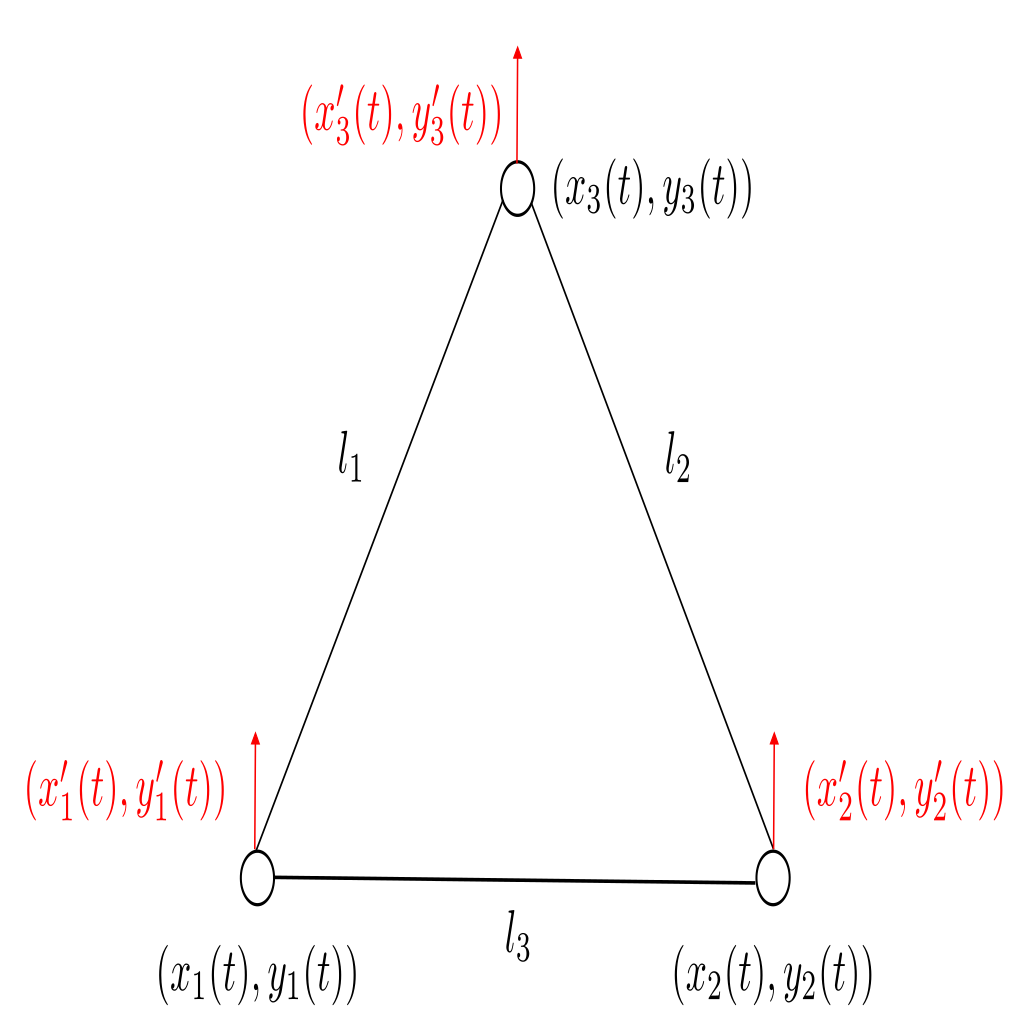
\includegraphics[width = 0.65\textwidth]{Chapter 2/13. inf_rigid_proof.png}
    \caption{A framework in $\mathbb{R}^2$, with some instantaneous velocity vectors at each node given in red.}
    \label{fig: inf_velocity}
\end{figure}

In Figure \ref{fig: inf_velocity}, we have a framework with three nodes, each defined by coordinates $(x_i(t), y_i(t))$ as well as their corresponding velocities given by $(x'_i(t), y'_i(t))$ for $i = 1,2,3$. As each point is fixed in the plane, the distances between each pair of nodes are constants, given as $l_i$ for $i = 1,2,3$.
\end{flushleft}

\begin{flushleft}
Therefore, we know that 
\vspace{-1 mm}
\[
\begin{split}
(x_1(t) - x_2(t))^2 + (y_1(t) - y_2(t))^2 = {l_3}^2 \\
(x_1(t) - x_3(t))^2 + (y_1(t) - y_3(t))^2 = {l_1}^2 \\
(x_2(t) - x_3(t))^2 + (y_2(t) - y_3(t))^2 = {l_2}^2
\end{split}
\]

Now, if we differentiate each equation with respect to $t$, we get 
\vspace{-1 mm}
\[
\begin{split}
2(x_1 - x_2)(x'_1 - x'_2) + 2(y_1 - y_2)(y'_1 - y'_2) = 0 \\
2(x_1 - x_3)(x'_1 - x'_3) + 2(y_1 - y_3)(y'_1 - y'_3) = 0 \\
2(x_2 - x_3)(x'_2 - x'_3) + 2(y_2 - y_3)(y'_2 - y'_3) = 0
\end{split}
\]

where we drop the dependence on $t$ for notational convenience. By factoring out the $2$, this set of equations can be written as
\vspace{-1 mm}
\[
\begin{split}
(x_1 - x_2, y_1 - y_2) \cdot (x'_1 - x'_2, y'_1 - y'_2) = 0 \\
(x_1 - x_3, y_1 - y_3) \cdot (x'_1 - x'_3, y'_1 - y'_3) = 0 \\
(x_2 - x_3, y_2 - y_3) \cdot (x'_2 - x'_3, y'_2 - y'_3) = 0
\end{split}
\]

Or more simply
%\vspace{-1 mm}
\[
(x_i - x_j, y_i - y_j) \cdot (x'_i - x'_j, y'_i - y'_j) = 0
\]

for all $i,j = 1,2,3$
\end{flushleft}

\begin{flushleft}
This observation allows us to impose conditions such that edge lengths and node distances are preserved when velocities are applied to a node, enabling us to study rigidity in even finer detail. With this in mind, let us formalize what we have just seen.
\end{flushleft}

\begin{definition}
Let $(G,\mathbf{p})$ be a framework where each node is on a differentiable smooth path parameterized by $t$ such that the position of each node is given by $\mathbf{p}_i(t)$ for all $i \in  V(G)$. Then \textit{instantaneous velocity} of the node $\mathbf{p}_i(t)$ is given by

\[
\mathbf{p}'_i(t) = \frac{d\mathbf{p}_i(t)}{dt}
\]

\noindent
for all $t$.
\end{definition} 

\begin{flushleft}
The instantaneous velocity of a node allows us to consider what happens to a framework as we attempt to deform it by applying some motion or force to every node. If we want a structure to be rigid in the conventional sense, then we enforce a condition such that the edges of the framework do not deform when such velocities are applied to the nodes of a framework. 
\end{flushleft}

\begin{definition}
\label{def: inf motion}
Let $(G,\mathbf{p})$ be a framework parameterized by $t$. 
\begin{itemize}
    \item An \textit{infinitesimal motion} of $(G,\mathbf{p})$ is given by $(\mathbf{p}_i - \mathbf{p}_j) \cdot (\mathbf{p}'_i - \mathbf{p}'_j) = 0$ for all $ij \in  E(G)$. 
    \vspace{-3mm}
    \item An infinitesimal motion is an \textit{infinitesimal rigid motion} of $(G,\mathbf{p})$ if $(\mathbf{p}_i - \mathbf{p}_j) \cdot (\mathbf{p}'_i - \mathbf{p}'_j) = 0$ for all $i,j \in  V(G)$. 
\end{itemize}
\noindent
Therefore, we obtain a system of equations, where the $(\mathbf{p}'_i - \mathbf{p}'_j)$ terms are unknown, and $(\mathbf{p}_i - \mathbf{p}_j)$ terms form our coefficients.
\end{definition}

\begin{flushleft}
As we saw when considering Figure \ref{fig: inf_velocity}, an infinitesimal motion of a framework is the assignment of an instantaneous velocities $\mathbf{p}'_i$ to nodes $\mathbf{p}_i$ such that the length of the edge $|\mathbf{p}_i - \mathbf{p}_j|$ remains constant for all edges $ij \in E(G)$. Analogously to before, if we can apply infinitesimal motions to the framework such that it preserves the distance between every node, then we have an infinitesimal rigid motion. 
\end{flushleft}

\begin{flushleft}
We have already seen that for a framework to be rigid in space, all of its motions must be rigid motions. A similar conclusion can be drawn here as well.
\end{flushleft}

\begin{definition}
\label{def: inf rigid}
Let $(G,\mathbf{p})$ be a framework parameterized by $t$. Then $(G,\mathbf{p})$ is \textit{infinitesimally rigid} if all of its infinitesimal motions are infinitesimal rigid motions.

\noindent
If a framework is not infinitesimally rigid, it is \textit{infinitesimally flexible}.
\end{definition}

% https://www.researchgate.net/figure/a-A-rigid-framework-which-is-not-infinitesimally-rigid-b-An-infinitesimally-flexible_fig5_220452659
\begin{example}
Let us look at a framework that is infinitesimally flexible.
\vspace{2mm}
\begin{figure}[htbp]
    \centering
    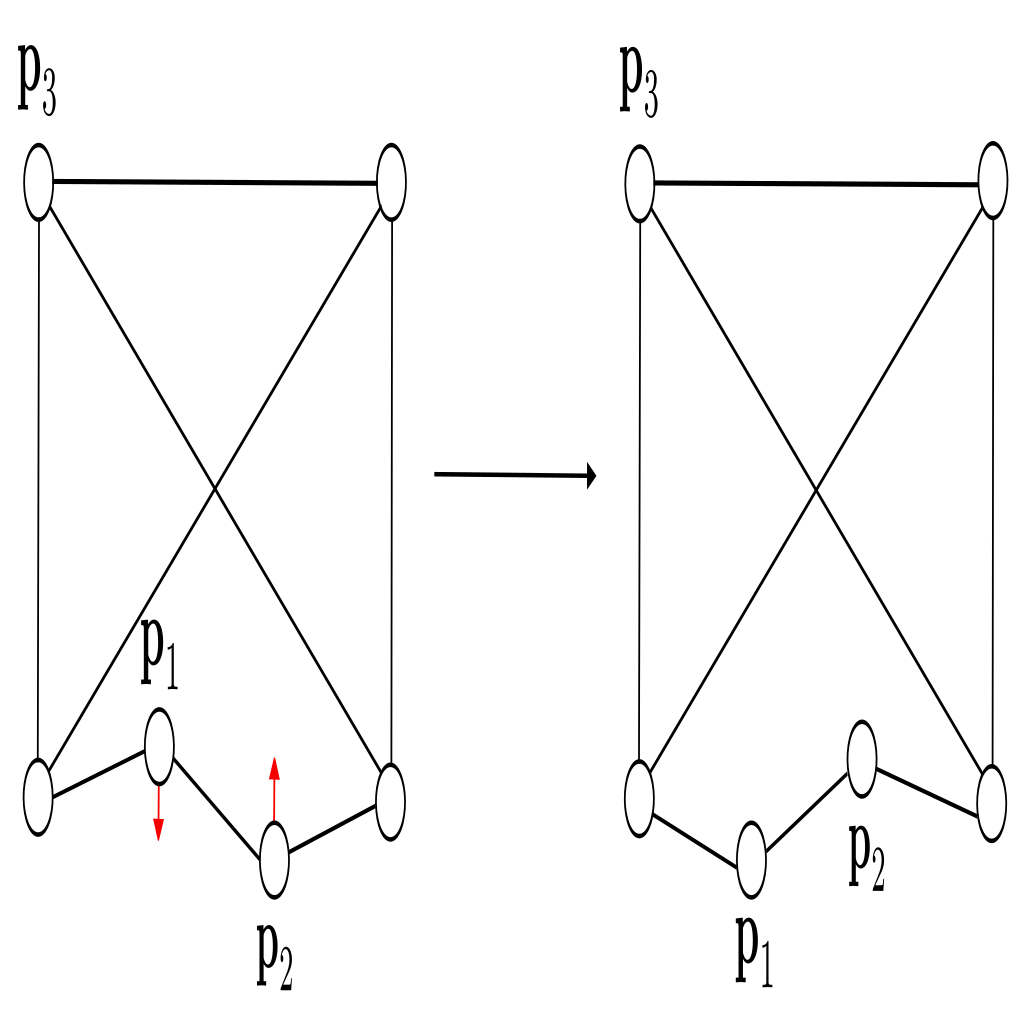
\includegraphics[width = 0.7\textwidth]{Chapter 2/10. not_inf_rigid_2.0.png}
    \caption{A framework that is not infinitesimally rigid}
    \label{eg: not inf rigid 2.0}
\end{figure}

\noindent
By applying instantaneous velocities to nodes $1$ and $2$ as shown in the framework on the left of Figure \ref{eg: not inf rigid 2.0}, we restructure the framework such that all the edge lengths are kept constant. This is shown in the framework on the right. However, the distance between nodes $1$ and $3$ have been altered. Therefore, this framework is not infinitesimally rigid.     

\begin{figure}[htbp]
    \centering
    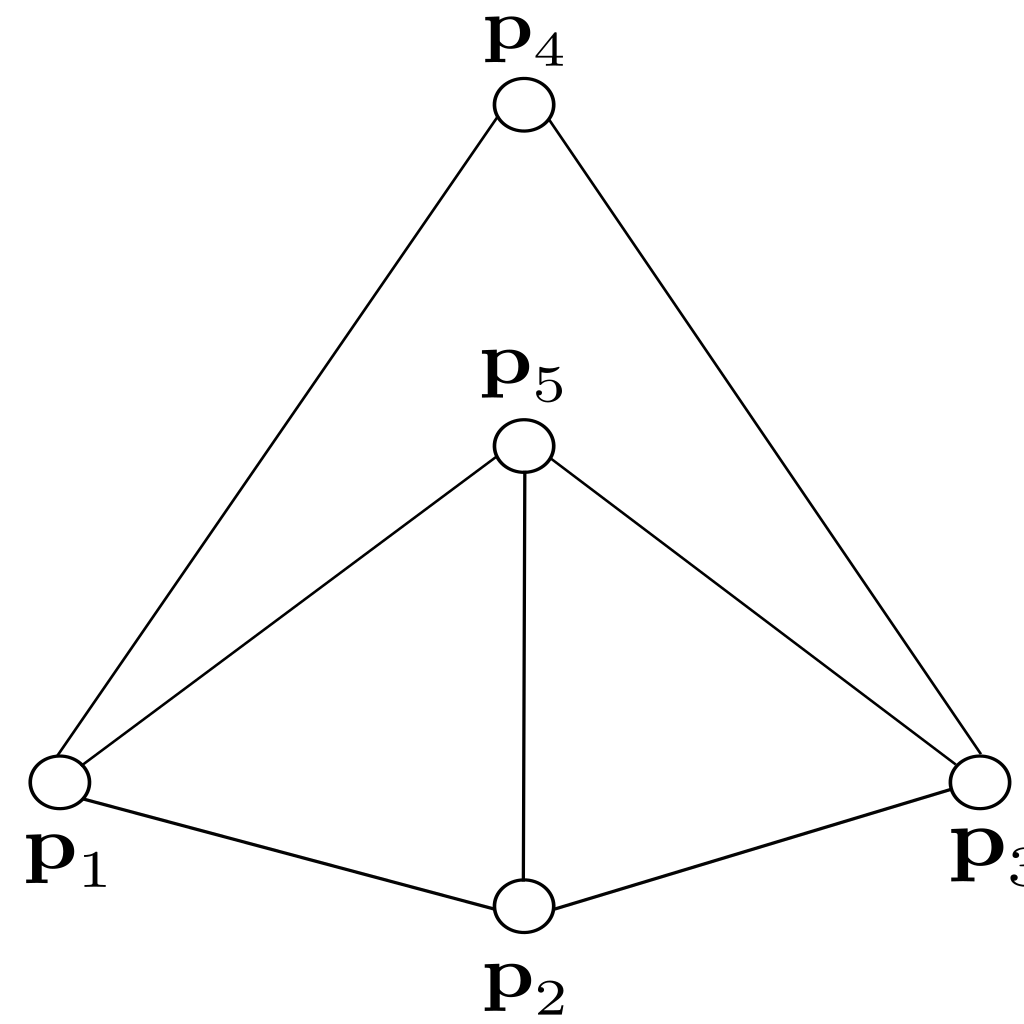
\includegraphics[width = 0.35\textwidth]{Chapter 2/11. inf_rigid.png}
    \caption{An infinitesimally rigid framework}
    \label{eg: inf rigid}
\end{figure}

\begin{flushleft}
Now consider the framework in Figure \ref{eg: inf rigid}. As we will soon see, triangular frameworks are infinitesimally rigid by a process known as a Henneberg construction of the first kind \cite{henneberg}. So this means that the framework can not be deformed by applying instantaneous velocities to nodes $1,2,3$  or $5$.     
\end{flushleft}

\begin{flushleft}
As the only way we can possible deform this framework is by applying some velocity to $4$, let us displace $4$ by an infinitesimal distance, say to the left without loss of generality. As our edges are of a fixed length, this will require edge $34$ to `pull' node $3$ upwards with the motion. As triangles $235$ and $125$ are known to be rigid, this causes the entire framework to rotate in an anti-clockwise fashion.
\end{flushleft}

\noindent
We already know that rotations are (infinitesimal) rigid motions, and so any displacement of the node $4$ results in an infinitesimal rigid motion. Therefore, we conclude that the framework in \hyperref[eg: inf rigid]{Figure 1.5} is infinitesimally rigid.
\end{example}

\subsection{Generic Rigidity}
We close this chapter on one last interesting way to classify rigidity. When studying configurations, we are interested in those that have nothing `special' about the way the points are arranged. Such configurations are known to be \textit{generic}.

\begin{flushleft}
To begin, we define a simpler result in order to get a feel for what we mean by not `special'.    
\end{flushleft}

\begin{definition}
Let $\mathbf{p} \in \mathbb{R}^d$ be a configuration. Then $\mathbf{p}$ is in \textit{general position} if any $d+1$ number of points do not lie in an $d-1$ dimensional affine space for $d>0$.
\end{definition}

\begin{flushleft}
Don't worry about what an affine space is as it is beyond the scope of this project! The definition essentially says that for a set of points to be in general position, we must \textbf{not} have:
\begin{itemize}
    \item Any two points that coincide at the same point when $d = 1$.
    \vspace{-3mm}
    \item Any three points that lie on the same line when $d = 2$.
    \vspace{-3mm}
    \item Any four points that lie on the same plane when $d = 3$.
\end{itemize}

And the pattern continues. This gives us a set of points that are spread out, making them more interesting to study.
\end{flushleft}

\begin{flushleft}
Genericity is a stronger condition than that of general position. The definition is as follows.
\end{flushleft}

\begin{definition}
A configuration $\mathbf{p}$ is \textit{generic} if the only polynomial with coefficients from $\mathbb{Q}$ that the coordinates of each point in $\mathbf{p}$ satisfies is the zero polynomial.
\end{definition}

\begin{flushleft}
A couple of examples of point-sets that are not generic by this definition include four points on a circle and a pair of points on a line that has a rational slope \cite{textbook}.

Finally, we conclude with what it means to be generically rigid.    
\end{flushleft}

\begin{theorem}
\label{def: generic rigid}
If $(G,\mathbf{p})$ is an infinitesimally rigid framework in $\mathbb{R}^d$, then $(G,\mathbf{q})$ is infinitesimally rigid for any generic configuration $\mathbf{q}$.
\end{theorem}

\begin{flushleft}
This is an extremely powerful result. If we can find a configuration $\mathbf{p} \in \mathbb{R}^d$, generic or not, such that $(G,\mathbf{p})$ is infinitesimally rigid, then Definition \ref{def: generic rigid} implies that for \textit{any} generic configuration $\mathbf{q}$, we can find a framework with the same underlying graph $G$, such that it is also infinitesimally rigid.
\end{flushleft}

\begin{definition}
A configuration $(G,\mathbf{p})$ is \textit{generically rigid} in $\mathbb{R}^d$ if it is infinitesimally rigid for any one configuration $\mathbf{p}$.
\end{definition}

\begin{flushleft}
With that, we conclude this introductory exploration into the definitions of rigidity. These concepts form the basis of everything that is to come in later chapters. 
\end{flushleft}

\begin{flushleft}
Our current objective is unravelling the multitude of theorems that surround the study of rigid graphs. The goal is to collect as many tools revolving around rigidity and circle packings as possible. By learning and invoking these ideas, we will be ever closer to understanding the structure of the special case of packings this project focuses on.
\end{flushleft}